\documentclass{beamer}
\usepackage{ctex}
\usepackage{graphics}
\usepackage{fancybox}
\usetheme{Warsaw}
\begin{document}
%%---------------------    Title Page And Table Of Contents  ----------------
\title{简略标题}
\subtitle{详细标题}
\author[1307402068李世旺]{李世旺}
\institute{苏州大学~数学院}
\date{$main~date = \Delta^\delta = $ \today}
\frame[plain]{\frametitle{~~~~~~~~标题栏}\titlepage}
\frame[plain]{\frametitle{Contents}\tableofcontents}
%%----------------------      section 1     ---------------------------
\section{section 1}
\begin{frame}\frametitle{标题1}
	\begin{enumerate}
\item The first item
\item The second item
\item The third item
\item The fourth item
	\end{enumerate}
\end{frame}
\begin{frame}
	\begin{description}[Second Item]
\item[First Item] Description of first item
\item[Second Item] Description of second item
\item[Third Item] Description of third item
\item[Forth Item] Description of forth item
	\end{description}
\end{frame}
\begin{frame}
	\begin{itemize}
\item The first item
\item The second item
\item The third item
\item The fourth item
	\end{itemize}
\end{frame}
%%----------------------      section 2     ---------------------------
\section{section 2}
\begin{frame}

\textbf{Step 1:} Compute the maximal suffix of $w$
with respect to $\preceq_l$ (say $v$) and the
maximal suffix of $w$ with respect to $\preceq_r$
(say $v’$).
\pause

\textbf{Step 2:} Find words $u$, $u’$ such that
$w = uv = u’v’$.
\pause

\textbf{Step 3:} If $|v| \le |v’|$, then output
$(u,v)$. Otherwise, output$(u’,v’)$.
\end{frame}
%%----------------------      section 3     ---------------------------
\section{section 3}
\begin{frame}
	\begin{itemize}
\item<1> $abcadcabc$
\item<1-2> $abcabcabc$
\item<1-2> $accaccacc$
\item<1> $bacbccbac$
\item<1,3> $cacdaccac$
\item<1-2> $caccaccac$
	\end{itemize}
\end{frame}
%%----------------------      section 4     ---------------------------
\section{section 4}
\subsection{subsection 1}
\begin{frame}

\alert{Alert on all slides}

\alert<2>{Alert on slide 2}

\alert<3>{Alert on slide 3}

\alert<1,3>{Alert on slides 1 and 3}

\alert<-2,4>{Alert on slides 1,2 and 4}

\end{frame}
\subsection{subsection 2}
\begin{frame}
\begin{block}{图表}
	\begin{tabular}{|c|c|c|c|}
	\hline
	& \textbf{header 1} &
	\textbf{header 2} & \textbf{header 4} \\
	\hline
	\textbf{header 4} &cell 1 & cell 2 & cell 3 \\
	\hline
	\textbf{header 5} & cell 4 & cell 5 & cell 6 \\
	\hline
\end{tabular}
\newline\newline
\begin{center}
\shadowbox{我的 beamer 文档测试成功!}
\end{center}
\end{block}
\end{frame}
\subsection{subsection 3}
\begin{frame}
\begin{columns}[t]
	\column{.5\textwidth}
		\begin{block}{插入图片 1 }
			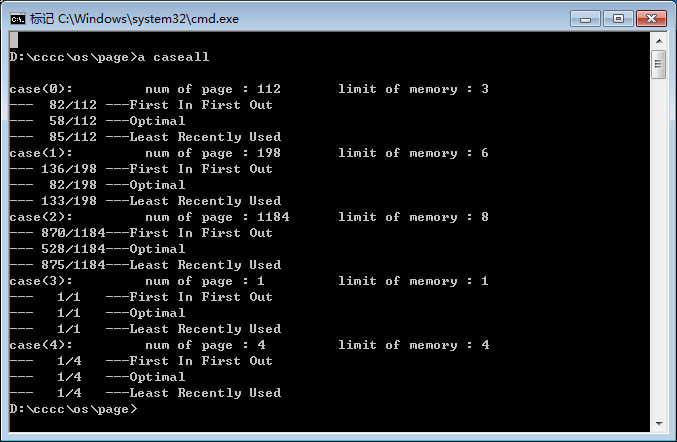
\includegraphics[height=3cm]{page.png}
			\newline
			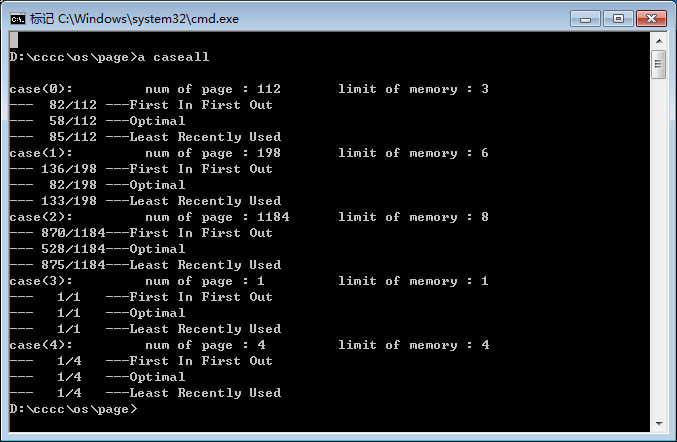
\includegraphics[height=3cm]{page.png}
		\end{block}
	\column{.5\textwidth}
		\begin{block}{插入图片 2 }
			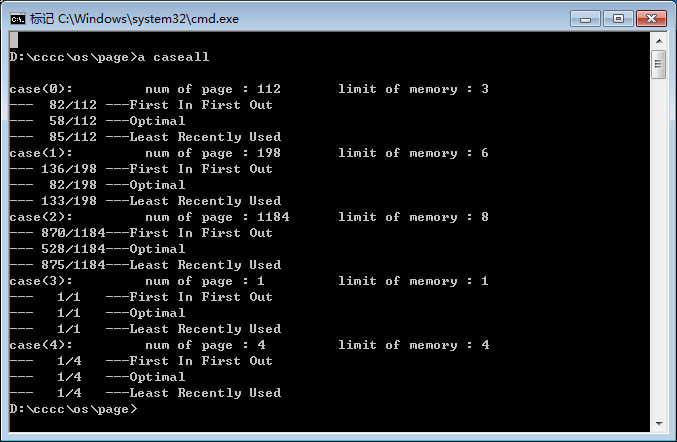
\includegraphics[height=3cm]{page.png}
		\end{block}
\end{columns}
\end{frame}
\subsection{subsection 4}
\begin{frame}
\begin{columns}[t]
	\column{.5\textwidth}
		\begin{theorem}{插入图片 1 }
			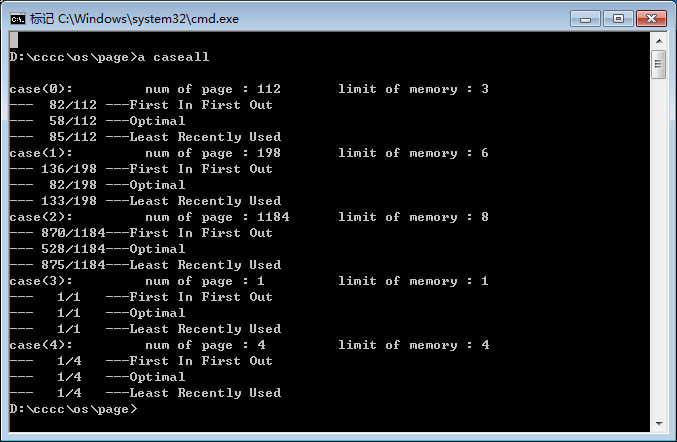
\includegraphics[height=3cm]{page.png}
			\newline
			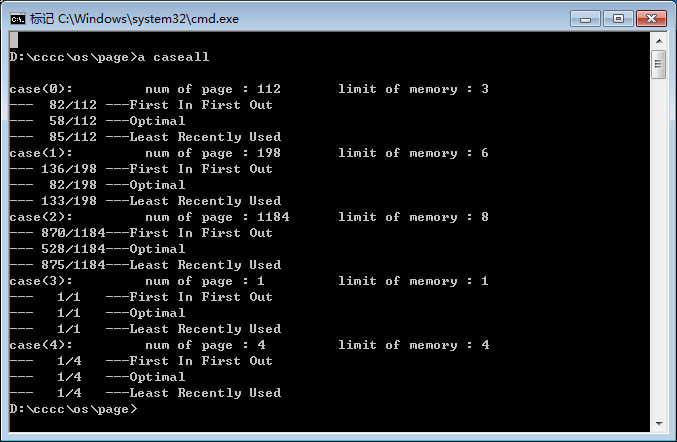
\includegraphics[height=3cm]{page.png}
		\end{theorem}
	\column{.5\textwidth}
		\begin{theorem}{插入图片 2 }
			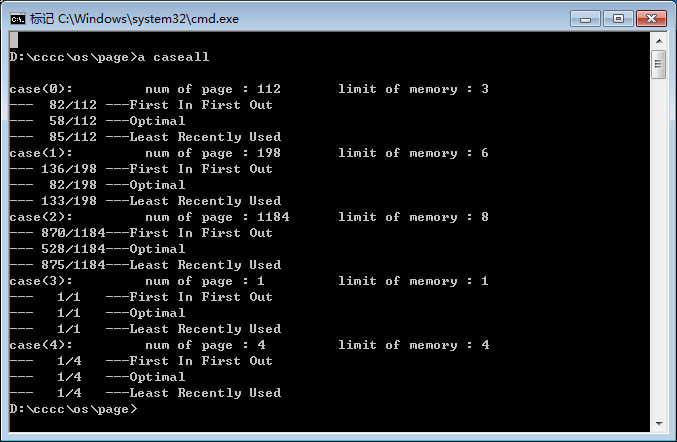
\includegraphics[height=3cm]{page.png}
		\end{theorem}
\end{columns}
\end{frame}
%%----------------------      End Of Document     ---------------------------
\end{document}